\chapter{Discussion}
\label{chap:discussion}


With the disks now fit, we may interpret our results. Since this project was based around the question of how environment influences protoplanetary disks, we would like to compare our best fit values to other disks, including to one other from the ONC \citep{Factor2017} as well as to others outside of it. We also consider how our results compare to modeling efforts.


% REWORK: I think somewhere before this section, ideally right at the start of the chapter, you should lay out a bunch of caveats about our abundances — particularly that they are derived from the MAJOR assumption the total disk gas mass will be 100x the dust mass derived from continuum emission.  It needs to be in everyone’s mind while they are reading about the modeling.  




\section{Reflections on the Fits}

As discussed in \S\ref{subsection:co_fit}, our attempts to fit the CO line were overwhelmed by the significant cloud contamination around the disk, resulting in physically-unreasonable best-fit values. If this run had converged to physical values, we would have used its disk mass results in the other runs, but since these results are not to be trusted, we instead continued to use the disks' mass values presented in \citet{Williams2014}, which were inferred from continuum emission.

% REWORK: be quantitative about "decidedly"
% REWORK all percentages: I’m not really interested in what percentage agreement is reached, but rather the significance of that agreement.  Do they agree to within 1-sigma, for example?  All of these percentage values need to be rewritten in terms of significance.
% The 50% figure is a little more interesting, but here I might just insert the actual values.  Something like: “The best-fit atmospheric temperature for HCO+ (xxx+/-xxx K) is significantly higher/lower than the corresponding value for HCN (xxx+/-xxx K), but this is at least somewhat expected…”
The \hco and HCN runs converged into impressive agreement, although the posteriors from the \hco line show smaller uncertainties than those of the HCN line. Both the \hco and HCN lines show molecular abundances in disk A that are almost two orders of magnitude than those in disk B (discussed later). The two lines' fits for disk A's outer radius agree to within around 1\% (although the HCN fit is significantly less certain than the \hco fit) and the lines' best-fit $q$ values agree to within 15\%. Atmospheric temperatures for disk A in both lines are large and significantly different, with the \hco line preferring a temperature 50\% greater than HCN's, but this is at least somewhat expected, as the two molecules are emitting from different regions of the disk and thus could reflect different regions of its temperature profile. In both lines, disk A's temperature structure power law index, $q$, is decidedly positive, although we expect this parameter to not settle with absolute certainty on a single value, since the observations don't have enough spatial resolution to constrain it tightly.


% REWORK: What does 'expected' mean? Useful?
Fits for disk B are systematically less well constrained, primarily in outer radius. This likely reflects the fact that it is smaller, unresolved, and more easily overrun by emission from features that were not modeled, such as cloud contamination, excess disk A emission, and emitting material shared by the two disks. The outer radius was most notably affected by these features, yielding somewhat bimodal posteriors in both \hco and HCN as the walkers sometimes tried to fit the outer features. As discussed in \S\ref{subsection:hcn_fit}, a posteriori cuts of the HCN model's MCMC chain limiting disk B's outer radius to $\geq$220 au - effectively manually choosing one of the posterior's two modes -  changed the best-fit parameters significantly, most notably leading the HCN fit's value for disk B's outer radius into agreement with \hco. It also pushed disk A's HCN abundance more than a full order of magnitude higher, and into nearly perfect agreement with results from HCN fitting in \citet{Factor2017}. Whether this is a reasonable thing to do is not clear to me.


That each disk's abundances are so different from one another is something of a surprise. Both disks have similar ratios of the two emitting molecules: disk A's \hco/HCN ratio of log abundances is 1.09, while disk B's is 0.95, becoming 1.21 for disk A and unity for disk B if the disk B radius cut is made.


We see in the HCN channel maps an area of significant flux coming from between disks around $ v = 9-11$ \kms. This may be region where the two disks are interacting, a possibility that our model does not take into account. The feature is less clearly present in \hco and invisible in CO, likely overrun by cloud contamination.





\section{Physical Structure}
% - Start off comparing basic stuff like masses and radii of your disks, so that we get the idea that relative to large populations of disks they are big and dense, but that relative to Sam’s disk they are comparable in mass/radius.

% REWORK: I’m not sure this is the study you want to talk about here, or how you want to present it.  A couple of thoughts:
% - You start off comparing the disks’ masses and radii to other disks in Orion, which is great.  Clearly apples to apples.
% - Next, you want to compare your disks to disks in low-mass SF regions.  Also great.  But to discuss how the properties of your disks compare to the properties of disks in low-mass SF regions, you need to compare the same data.  So you’d want to look for a study (and there are lots! some of which you talk about below!) that compiled disk masses based on mm continuum measurements, assuming 100:1 gas:dust mass ratio like Rita did.
% - The study you’re referencing here (Miotello2016) is really great and important!  But I think you want to discuss it in the context of the assumptions you made and why they might not be correct.  Specifically, this study provides evidence that 100:1 may not be a valid assumption for the gas:dust mass ratio in protoplanetary disks.
% So, all good stuff, but just organized weirdly.  I think you should also describe a bit more of the methodology of how the authors “analyze several CO isotopologues” — this is a nonstandard (but very interesting!) method that involves comparison of data with radiative transfer models of a large grid of generic disk models, so you should say a bit more about what they did so that your reader can better interpret it.  


% REWORK: One thing you need to make sure to include in any discussion of disk mass ranges is a discussion of sensitivity limitations.  Are there disks with masses less than 1 M_Jup?  Probably!  Are they detectable?  Nope.  Also, the sensitivity limits are lower for low-mass SF regions than for high-mass, simply because they’re closer, which is another important caveat that is currently missing from your discussion. 



To get a sense of how these disks' physical characteristics (i.e. mass and radius) compare to other protoplanetary disks, it is useful to compare our results to other disks in the Orion Nebula Cluster, as well as others in low-mass star forming regions (SFRs). For these comparisons, we again draw on the disks' inferred gas mass measurements made by \citet{Williams2014}, which carry with them significant uncertainty on account of the 100:1 assumed gas:dust ratio (as described in \S\ref{chap:introduction}). As such, the values we use for the masses of disk A and disk B are 0.075 M$_\odot$ and 0.029 M$_\odot$ (78.66 and 29.88 Jovian masses), respectively. Our best-fit values for radii from the MCMC models were around 337 and 145 au, respectively.


% REWORK: "“of the disks’ radial extents, [based on…]” (i.e., say how they estimated the radial extent, so that it is clear when you’re comparing apples to apples and when you’re not)."
% REWORK: Check that the first Factor2017 reference prints correctly using the trick citet syntax
% REWORK: percentages to sigmas
In the survey of ONC proplyds that originally provided these data, \citet{Mann2014} calculated initial disk masses and the semi-minor and -major axes of the disks, approximate measures of the disks' radial extents. The survey had a sensitivity limit of  Disk A in the present system was, by their measure, the most massive disk in the study, 75\% more massive than the study's next most massive disk, d216-0939 \citet[which was the subject of][]{Factor2017}; disk B was the fifth most massive. Disk A had the study's fourth largest semi-major axis\footnote{The authors' measurement of disk A's semi-major axis, at 268 au, is 20\% smaller than our fit measurements. The survey's reported semi-major axis for d216-0939 was also smaller than the fit value in \citet{Factor2017}, though by only 6\%.}. The authors did not fit disk B's radial extent; however, our measurement of 145 AU would make it the eleventh (out of 22) largest disk in the survey. Thus, disk A is on the very high end of the study's mass and radius range, while disk B is apparently quite dense and of median radial extent.

% REWORK (on "it's not terribly useful"): It is!  You can make the same 100:1 assumption as the other studies to compare the data.  This is a great study to include in the comparison, since it is also a high-mass region.
% On the topic of disks in high-mass SFRs, \citet{Eisner2018} conducted a particularly comprehensive survey of disks in $\sigma$ Ori, a young cluster in the ONC, north of M42 and M43.

However, all these disks are in the Orion Nebula Cluster, a high-mass SFR. We would also like to understand how these disks compare to disks in low-mass SFRs. Several surveys have been made of protoplanetary disks in low-mass SFRs.

\citet{Eisner2018} conducted a particularly comprehensive survey of 104 detected disks in M43 within 0.14 pc of $\theta^1$C, measuring the disks' dust masses (from continuum flux) and radii (from the half-max half-width of the major axis of 2D Gaussian fits to the disks), and comparing their results to similar measurements from other surveys of disks in low mass SFRs. These comparisons are summarized in fig.\ref{fig:eisner18_disk_properties}, showing the distributions of masses and radii of disks in each survey. From them, we see that the M43 disks are characteristically denser and radially truncated, as shown by the ONC track's relatively high position on the mass plot and relatively low position on the radius plot. By inferring the dust masses of the present binary's disks using the 100:1 gas/dust ratio (yielding masses of around 250 M$_\oplus$ and 95 M$_\oplus$ for disk A and B, respectively) and recalling our fit radii (around 335 and 145 au, respectively), we may place these two disks on these plots and find that they are far more massive than the other ONC disks and that disk A is more massive than any of the disks in all the surveys. However, while the ONC disks in this plot exhibit an atypically high density (the highest-mass disks have mass:radius ratios of around 1.5 M$_\oplus$/au) relative to the other survey's disks (which are closer to of order 0.5 M$_\oplus$/au), disk A and B land at 0.75 and 0.65, respectively. This indicates that, while they are still somewhat more dense than the disks from low-mass SFRs, they are not as dense as the disks in M43 and do not show the same radial truncation found in the M43 disks.



\begin{figure}[h!]
  \centering
    \hspace*{\fill}%
    \subcaptionbox{Disk mass distribution across surveys}{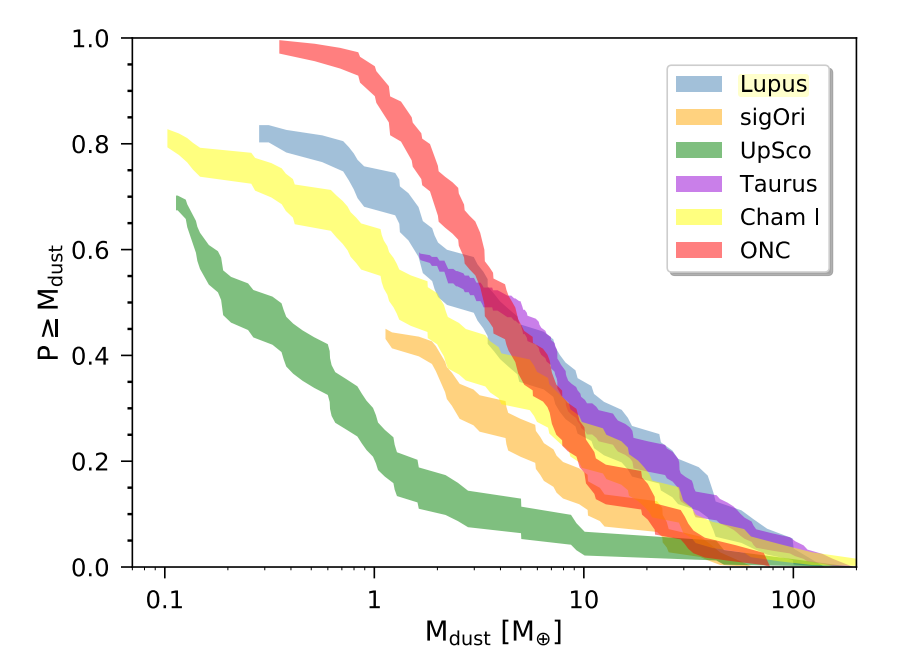
\includegraphics[width=0.5\linewidth]{dust_mass_dist_Eisner18.png}}%
    \subcaptionbox{Disk radius distribution across surveys}{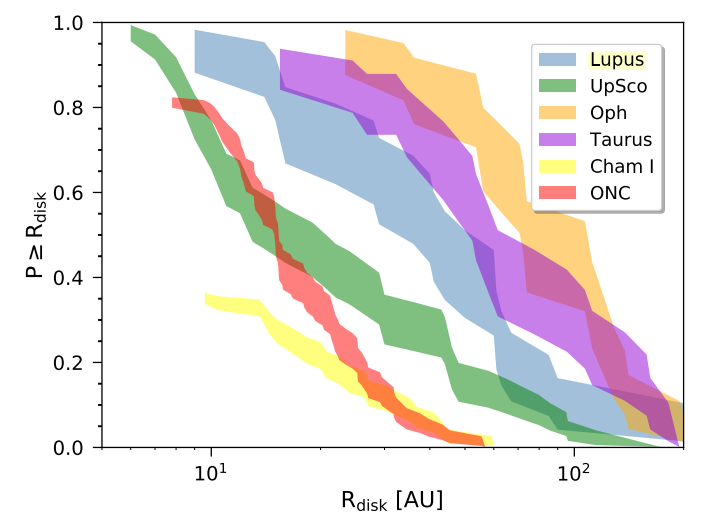
\includegraphics[width=0.5\linewidth]{dust_radius_dist_Eisner18.png}}%
    \hspace*{\fill}%
    \caption{Plots of disk masses and radii frequencies \citep{Eisner2018}. Blah blah blah}
    \label{fig:eisner18_disk_properties}
\end{figure}


\citet{Ansdell2016} and \citet{Ansdell2018} characterized the mass (both dust and gas) and radius distributions of protoplanetary disks in Lupus using CO isotopologues and continuum emission. To derive gas masses, they assumed a CO/H$_2$ ratio of $10^{-4}$ and then used the isotopologues' ratios to find total masses. Of these gas masses that they were able to constrain, they found disks to range from around 1-10 Jovian masses.


\citet{Williams2019} surveyed 279 disks in $\rho$ Ophiuchus and found some stuff from dust emission. Probably good to screengrab some of their plots


% REWORK: Choose unit for masses: odot, oplus, Jovian
In \citet{Miotello2016}, the authors analyze several CO isotopologues to retrieve the gas masses (rather than by inferring it from continuum emission) of 34 protoplanetary disks in Lupus. In it, they report masses that are systematically lower than the masses that would be predicted by the ISM GDR of 100:1, providing evidence that the ISM value is likely not a valid general assumption for gas/dust ratios in protoplanetary disks.

The resulting gas masses ranged from $10^{-5}$ to $10^{-3}$ M$_\odot$, with the most massive at 1.5 $\times 10^{-3}$ M$_\odot$ (1.6 Jovian masses). Since the disks were not spatially resolved, radii were not measured, so no comparison of their compactness can be made.









\section{Chemical Structure}



\subsection{Comparison to Modeling}
% You might consider starting by describing the models, so that we know what to expect.  Talk about what the models predict, then talk about how your disks fit in with those predictions.

% REWORK: There’s more to this field than one series of papers by Catherine Walsh!  Need to represent the whole diversity of the field.  Look up papers by Yuri Aikawa, Ted Bergin’s group, 

We may also compare these abundances to theoretical modeling efforts. \citet{Walsh2010} developed radial and vertical chemical models for an isolated protoplanetary disk around a T-Tauri star (a system with physical parameters similar to the famous TW Hya and its disk), studying molecular abundance distributions throughout the disk for molecules within ALMA's reach. They showed that log abundances in their models for \hco varied from $-8$ to $-12$, $-7$ to $-12$ for HCN, and $-4$ to $-9$ for CO. The authors then built on this model by adding robust modeling of externally-driven UV and X-ray ionization \citep{Walsh2012} and applying it to the same disk system, this time with an O star nearby providing ionizing photons \citep{Walsh2013}. They then make the same molecular abundance distribution maps as before (see Fig. \ref{fig:walsh-abundance-profs}). The authors note that, in their model photoionized disk, \hco column density increases by a factor of 6.3 relative to the isolated disk, whereas HCN and CO column densities remain constant through ionization\footnote{This would be useful if we had an estimation of what the \hco/HCN ratio would be in these two disks. They do have column density ratios in Walsh13; is it reasonable to say (I guess it would have to be in the case of optically thin emission) that col dens $\propto$ abundance? If that were the case then we'd be golden.}. They also note that the ionized disks have much higher gas temperatures, $\gg$ 50 K, which is consistent with our findings.


Although our modeling assumes a constant chemical abundance across the whole disk, these models offer a way to confirm that our results are within the predicted ranges, despite the fact that the \hco abundance is significantly higher than the values found by other studies.




\begin{figure}[t]
  \hspace*{\fill}%
  \subcaptionbox{CO abundances}{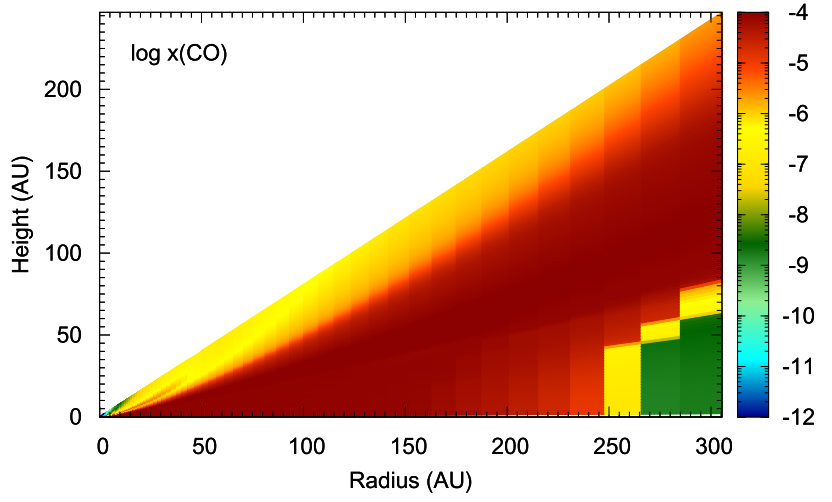
\includegraphics[width=0.33\linewidth]{walsh10_Xco.png}}%
  \subcaptionbox{\hco abundances}{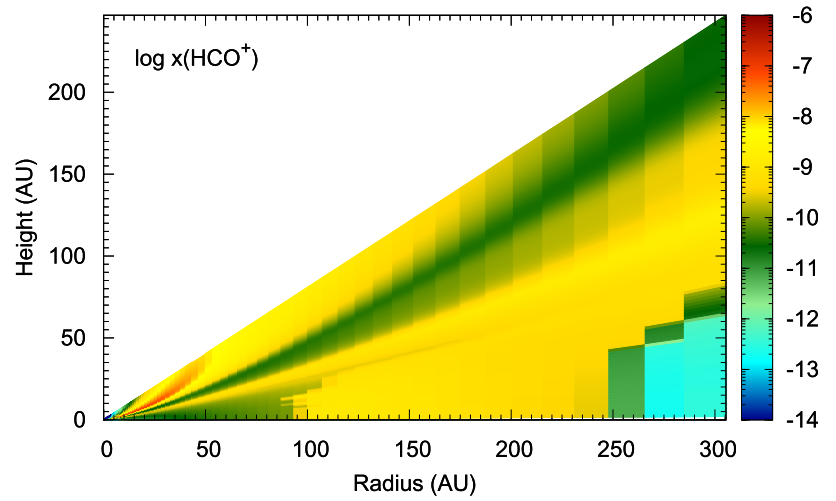
\includegraphics[width=0.33\linewidth]{walsh10_Xhco.png}}%
  \subcaptionbox{HCN abundances}{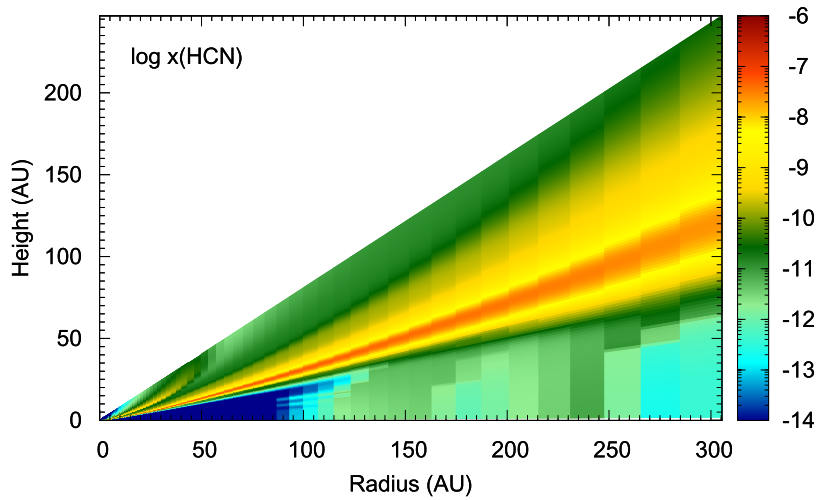
\includegraphics[width=0.33\linewidth]{walsh10_Xhcn.png}}\vfill%
  \subcaptionbox{CO abundances}{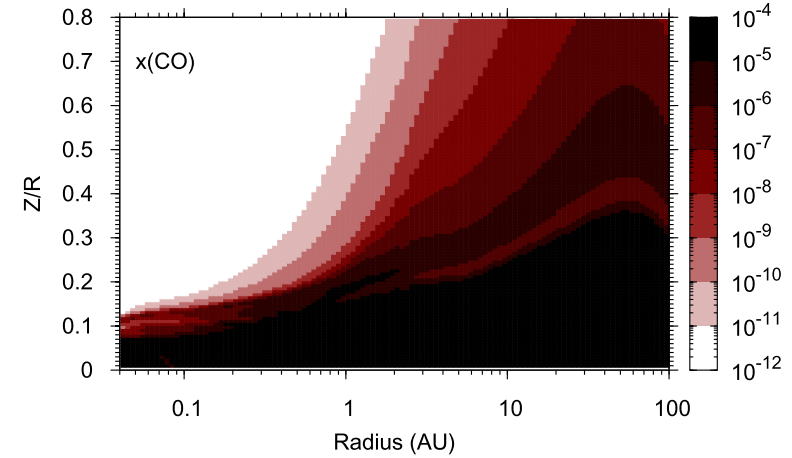
\includegraphics[width=0.33\linewidth]{walsh13_Xco.png}}%
  \subcaptionbox{\hco abundances}{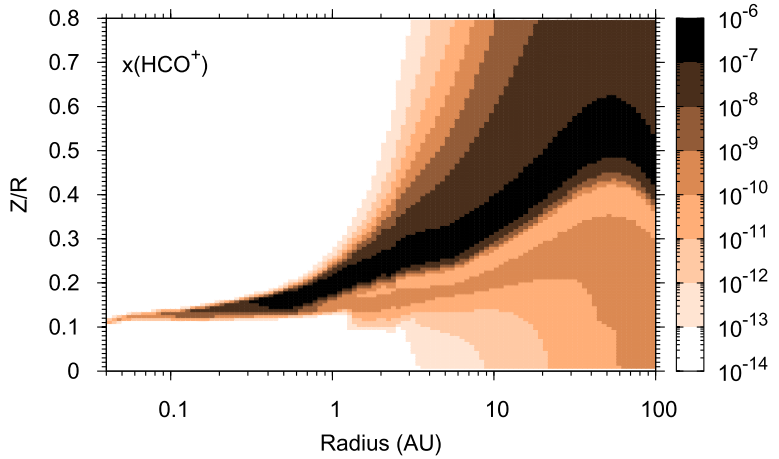
\includegraphics[width=0.33\linewidth]{walsh13_Xhco.png}}%
  \subcaptionbox{HCN abundances}{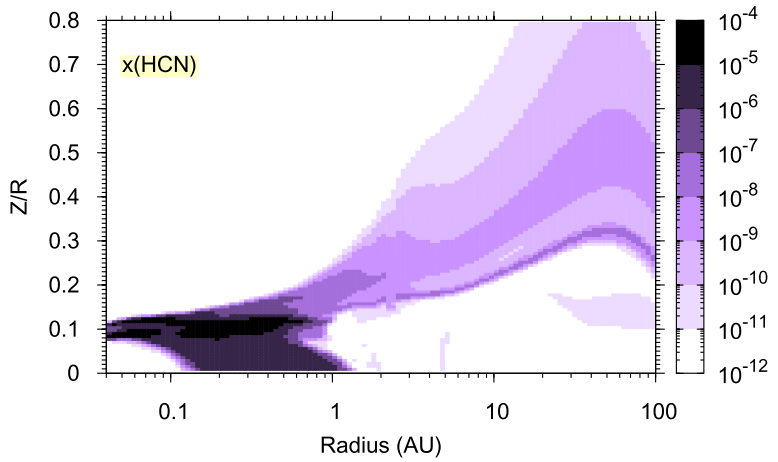
\includegraphics[width=0.33\linewidth]{walsh13_Xhcn.png}}%
  \hspace*{\fill}%
  \caption{Models showing radial and vertical distributions of CO, \hco, and HCN in a simulated disk around a T-Tauri star. The top row shows the profiles of isolated disks \citep{Walsh2010}, while the bottom row shows the profiles of disks being irradiated by a nearby O star \citep{Walsh2013}. Note that bottom row is on a log scale and only covers the inner 100 AU of the disk, while the top row is linearly scaled and shows a 300AU stretch. \textit{It seems like only having one of these sets of images would make more sense.}}
  \label{fig:walsh-abundance-profs}
\end{figure}



Some references:
- Observations and modeling of gaseous protoplanetary disks (2008): https://iopscience.iop.org/article/10.1088/0031-8949/2008/T130/014011/pdf
- CHEMICAL NETWORK REDUCTION IN PROTOPLANETARY DISKS: https://arxiv.org/pdf/1901.04888.pdf
    - Fig 4 predicts low (-12) X_HCO+
- The chemistry of disks around T Tauri and Herbig Ae/Be stars: https://arxiv.org/pdf/1803.09450.pdf
    - Shouldn't see differences in HCN/HCO+/CS abundances between disks around TT and HA/HB stars
- AN ALMA SURVEY OF DCN/H13CN AND DCO+/H13CO+ IN PROTOPLANETARY DISKS: https://arxiv.org/pdf/1701.01735.pdf
    - Seems cool but idk what's going on
- MULTIPLE PATHS OF DEUTERIUM FRACTIONATION IN PROTOPLANETARY DISKS: https://arxiv.org/pdf/1803.02498.pdf
    - How DCO+ gets formed. Interesting, but not critically relevant
- Intro to Astrochemistry (textbook): https://link.springer.com/content/pdf/10.1007%2F978-4-431-54171-4.pdf
- Physical and chemical structure of planet-forming disks probed by millimeter observations and modeling: https://arxiv.org/pdf/1402.3503.pdf
    - A nice 2014 review, but not sure what to take away from it
- The first multi-dimensional view of mass loss from externally FUV irradiated protoplanetary discs (2019): https://arxiv.org/pdf/1903.03644.pdf
- The ALMA Lupus protoplanetary disk survey: evidence for compact gas disks and molecular rings from CN (2018): https://arxiv.org/pdf/1811.03071.pdf


- Stellar disk destruction by dynamical interactions in the Orion Trapezium star cluster (2015): https://arxiv.org/pdf/1511.08900.pdf
- External photoevaporation of protoplanetary discs in Cygnus OB2: linking discs to star formation dynamical history (2019): https://arxiv.org/pdf/1902.04586.pdf

- Slideshow from Oberg: https://www.cfa.harvard.edu/sma/events/smaConf/posters/images/Oberg_SMA_archive.pdf
  - p. 17: chemical depletion of CO


\subsection{Comparison to Other Obsevations}
% you can do a pretty detailed comparison of your disk vs. Sam’s disk (in the table, yes, but also discussed in words in the text) and then you can compare with disks from low-mass SF regions as well (again, you’ve got a lot of the seeds of that discussion here).



% REWORK: "In terms of content, this is a great start, but how exhaustive is it?  I think you need to specify exactly what you’re doing with this table, and how you decided which disks to compare with and which ones not to.  The French group (Guilloteau, Dutrey, and others) would be very upset that you didn’t include any of their work, for example!  I really like the idea behind this table, but I think you need to go big or go home — make sure you’re specific about what is included in the table, and then make sure you are thorough about including all the relevant studies."
\begin{table}[ht!]
  % \centering
  \begin{threeparttable}
    \caption{Disk Parameter List}
    \label{table:comparisons}
    \renewcommand{\arraystretch}{1.2}
    \begin{tabular}{l l l c c c }
      \toprule \toprule
      %\multirow{2}{*}{Parameter} & \multirow{2}{*}{Disk A}    & \multicolumn{2}{c}{Disk B} \\
      Reference                             & Source     & Line          & $q$ & log X$_\text{mol}$ & Atms. Temp\\
      \midrule %\midrule
      \multirow{3}{*}{This study}           & d253-1536a & \hco(4-3)      & $0.66$  & $-7.96$         & $151$  \\
                                            & d253-1536a & HCN(4-3)       & $0.72$  & $-7.62$         & 140  \\
                                            & d253-1536a & CO(3-2)\tnote{a} & $0.40$  & $[-4]$        & 1  \\
      \hline
      \multirow{3}{*}{\cite{Factor2017}}   & d216-0939  & \hco(4-3)      & $0.17$  & $-10.08$        & 190  \\
                                           & d216-0939  & CO(3-2)        & $-0.33$ & $[-4]$          & 70  \\
                                           & d216-0939  & HCN(4-3)       & $-0.18$ & $-6.7$          & 19  \\
      \hline
      \multirow{2}{*}{\citet{Flaherty2015}}& HD163296   & CO(3-2)        & $-0.22$ & $[-4]$          & 94  \\
                                           & HD163296   & CO(2-1)        & $-0.27$ & $[-4]$          & 79  \\
      \hline
      \citet{Hughes2008}\tnote{b}           & A bunch    & CO(3-2)        &  -    & $[-4]$          & -  \\
      \hline
      \citet{Rosenfeld2012}\tnote{b}        & V4046 Sgr  & $^{12}$CO(2-1) & $-0.63$ & $[-4]$           & -  \\
      \hline
      \citet{Dutrey2014}        & GG Tau A  & Continuum & $-1.1$ & $NA$          & 13.8  \\
      \hline
      \citet{Flaherty2017}\tnote{c}         & HD163296   & DCO$^+$(3-2)   & $[-2.22]$ & $-10.79$      & [94]  \\
      \hline
      \citet{Zhang2017}                     & TW Hya     & $^{13}$C$^{18}$O(3-2), C$^{18}$O(3-2)  & $-0.47$ & -7.96 & 151  \\
      \hline
      \citet{Flaherty2018}\tnote{d}         & TW Hya     & CO(6-5, 3-2, 2-1) & $-0.46$ & $[-4]$       & 31  \\
      \bottomrule
    \end{tabular}
    \begin{tablenotes}\footnotesize
      \item[*] Values in [brackets] were fixed during fitting.
      \item[\dagger] Since there is not a convention about whether a negative value of $q$ indicates a radially decreasing or increasing temperature structure (in other words, whether or not $q$ is implicitly negative), some of these values have the opposite sign of the value reported in their article. When this is the case, it indicates that, in that original paper, atmospheric temperature was defined such that T$_{atms} \propto r^{-q}$. In our work, and in all the values given here, it is the case that T$_{atms} \propto r^{q}$, meaning that a negative value of $q$ leads to temperature decreasing with radius.
      \item[a] This result is being presented for completeness (and to allow for the chance that something changes dramatically in coming runs REWORK), but since its T$_{atms}$ clearly got stuck, it is not a useful result for comparison and will not be discussed.
      \item[b] \cite{Rosenfeld2012} didn't fit for tatms
      \item[c] In \citet{Flaherty2017}, they fit three rings, and consequently have three slightly different values for each parameter. The values reported here are for their middle ring, although the three do not vary significantly from one another. Additionally, T$_{atms}$ and $q$ were fixed at values found for CO(3-2) in \citet{Flaherty2015}, and only X$_\text{mol}$ was fit for.
      \item[d] \citet{Flaherty2018} developed several models, with different morphological structures. The results presented here are drawn from their simplest (fiducial) model.
    \end{tablenotes}
  \end{threeparttable}
\end{table}

% TO ADD:
% Dutrey 2014: Disks in CG Tau: https://www.nature.com/articles/nature13822#abstract




In Table \ref{table:comparisons} we compare our results to those from other studies that have modeled line emission from protoplanetary disks. The most immediately relevant of these is the work by \citet{Factor2017}, in which they use a similar modeling technique to characterize another ONC proplyd from the same survey as our binary, and thus represents the only other disk studied in this way that is also in a high-mass star forming region. The others are well-studied disks in low-mass regions. We may compare our temperature profiles and abundance to these other systems and look for variations from expected values.

Comparing our results for disk A to these other studies, we can see that our atmospheric temperatures in \hco(4-3) and HCN(4-3) are consistent with the results of the \hco fit in \citet{Factor2017}. They are, however, significantly higher than any other study's fit.
% FROM SAM: The slightly positive value of q derived for HCO+ is most likely due to the effect of observing an optically thin line of a molecule that freezes out in the midplane. As Schwarz et al. (2016) explain in a similar investigation of the molecular line emission from the disk around TW Hya, a flat temperature profile is expected in the case where most of the detected emission originates from the layer of the disk just above the freeze-out temperature.


Additionally, our temperature structures for both \hco and HCN are solidly positive, reflecting a structure that increases with radius. As with the atmospheric temperature, this is contrasted by all other results, which have moderately negative values, save again for that of the \citet{Factor2017} \hco line, which is also positive but less so than in our fits. Our positive values stand somewhat in contrast to the $q$ value of $-0.5_{-0.1}^{0.2}$ predicted by \citet{Dartois2003} for a geometrically flat, optically thin disk.
% REWORK on "stand somewhat in contrast...": "I’d remove the “somewhat,” and add some information about why you expect the decreasing temperature structure.  Then you could talk about some of the methodology that is likely to be influencing your result: spatially unresolved systems, assumptions about freeze-out and photodissociation that might lead the algorithm to artificially require increased temperatures just to have any molecular emission at large radii, etc."


Our molecular abundances for each disk vary from those reported in the \citet{Factor2017} paper, the only other study to do forward-modeling of \hco emission using a ray tracing code. In it, they report finding canonical values for the \hco line (log X$_{\text{HCO}^+}$ = $-10.04$) and unexpectedly high values for the HCN line (log X$_{HCN}$ = $-6.7$), contrasted by our findings of $-8.36$ and $-7.62$, respectively\footnote{Although, as described above, removing samples with large outer radii for disk B pushes disk A's HCN abundance to -6.98, within the uncertainties of their HCN fit.}.





Binaries in the ONC (2012) (not radio): https://www.aanda.org/articles/aa/pdf/2012/04/aa18314-11.pdf
Binaries in Taurus (2012): Harris2012
Binaries in Taurus (2019): Akeson2019
Binaries in rho Ophiucus (2014): Akeson2014 (49 systems, 63 stars)
Binaries in rho Ophiucus (2017): cox2017
GG Tau A: Dutrey2014
% In close (\textless100 au) binary systems, it is predicted \citep{someone} that circumstellar disks should develop around each star in addition to an outer circumbinary disk. \citet{Dutrey2014} used high-resolution ALMA observations to reveal such a system around a heirarchical triple system (where a binary pair is one element of a larger binary) revealed complex interactions between the various disks. However, since both tiers of this system are very close (the outer binary has an apparent separation of 35 au, while the inner pair are separated by just 4.5 au), the system is not entirely comparable to our present binary.



We must also consider the fact that these disks are in a binary. Several surveys have observed a number of binaries in various regions, most notably in Taurus and $\rho$ Ophiucus. Since these regions are low-mass SFRs, they are qualitatively different environments than the ONC, but provide us with a good starting point to compare to.

It has long been known \citep[and references contained therein][]{Jensen1995} that close (\textless50-100 au) binaries have lower combined fluxes than wider binaries or single stars.

\citet{Harris2012} observed 23 multiple-star systems in Taurus using the Submillimeter Array. In it, they found a strong anticorrelation between system brightness and projected separation between components, with wide pairs (\textgreater300 au) showing similar brightness to that of two single stars, while tight pairs (\textless30 au) suffer a $t\times$ decrease from the equivalent sum of individual brightnesses; however, the presence of circumbinary disks made the system significantly brighter (Fig.\ref{fig:harris2012_binary_brightnesses}). \citet{Akeson2019} built on these results with an ALMA survey of additional binaries in Taurus, developing a sample of 151 sources with resolved millimeter detections, 99 of which were in binary systems\footnote{The fact that this number is odd just reflects that at least one of the binaries had an undetected secondary member.}. From this sample, they found that disks around the binaries' primary (more massive) star contributes, on average, 62\% of the disks' total combined mass, although values for this ratio spanned three orders of magnitude. They also developed \citet{Harris2012}'s observation that tighter binaries led to lower fluxes, finding that, as a function of stellar mass, disks in binaries have systematically lower masses than their isolated counterparts, and that this mass truncation is more apparent in tighter binaries (see Fig.\ref{fig:taurus_binaries}). The absence of a significant population of circumbinary disks in the sample suggests that they are either not common or quickly (\textless1-2 Myr) dissipated. Finally, they found that M$_\text{disk}$/M_$\star$ for the primary and secondary stars are correlated in close systems but anticorrelated in wide systems, but that the rough correlation between disk mass and stellar mass shown in \citet{Andrews2013} did not hold in their sample.


\begin{figure}[t]
  \subcaptionbox{Harris2012}{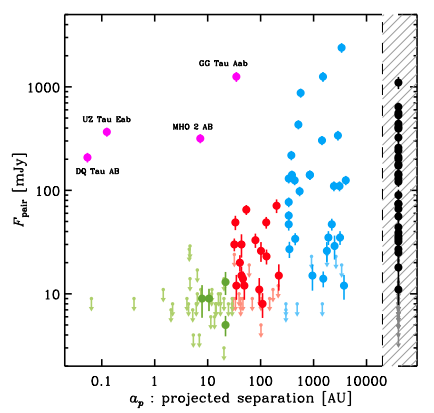
\includegraphics[width=0.33\linewidth]{harris2012_binary_brightnesses.png}}%
  \subcaptionbox{Harris2012}{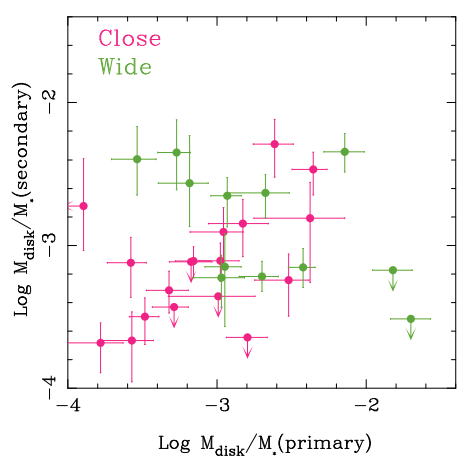
\includegraphics[width=0.33\linewidth]{akeson2019_binary_mass_ratios.png}}%
  \subcaptionbox{Harris2012}{\includegraphics[width=0.33\linewidth]{Akeson2019_binary-stellar-masses.png}}%
  \caption{\textit{Kaplan-Meier estimator of the cumulative distribution of stellar masses for our statistical analysis sample, displayed in various ways. In this and the following plots, the shaded region shows the ±1? confidence region around the estimated distribution. The difference between primary and secondary star stellar masses is more prominent among the wider binaries.}}
  \label{fig:taurus_binaries}
\end{figure}



Disks in binary pairs have also been surveyed in the $\rho$ Ophiucus region. \citet{Akeson2014} studied 17 pairs with separations ranging from 101-990 au using ALMA, designed to measure the systems' masses. In it, they found no correlation between disk mass and stellar masses, matching the results from the studies of Taurus binaries above. \citet{Cox2017} followed with a survey targeting 63 total sources, comprised of 11 binaries, three triple systems, and 34 single sources; this also represented the first survey to characterize disk radii. In it, they, like \citet{Harris2012,Akeson2019}, found significantly lower fluxes from sources in binaries than isolated ones, and found that the disks' radii also exhibited systematic truncation. They note that this truncation is either due to tidal interactions between the disks or reflects a natural limit on the radii of disks in binaries, inherent to the disks' formation process, and that these decreased fluxes can be generally interpreted as being proportional to decreased masses. The authors also compared their sample to a $Spitzer$ survey of disks in Taurus \citep{Rebull2012 REWORK GET THIS REF}, and found that fluxes from disks in $\rho$ Ophiucus are typically dimmer than those in Taurus.


 \begin{figure}[t]
   \hspace*{\fill}%
   \subcaptionbox{\hco abundances}{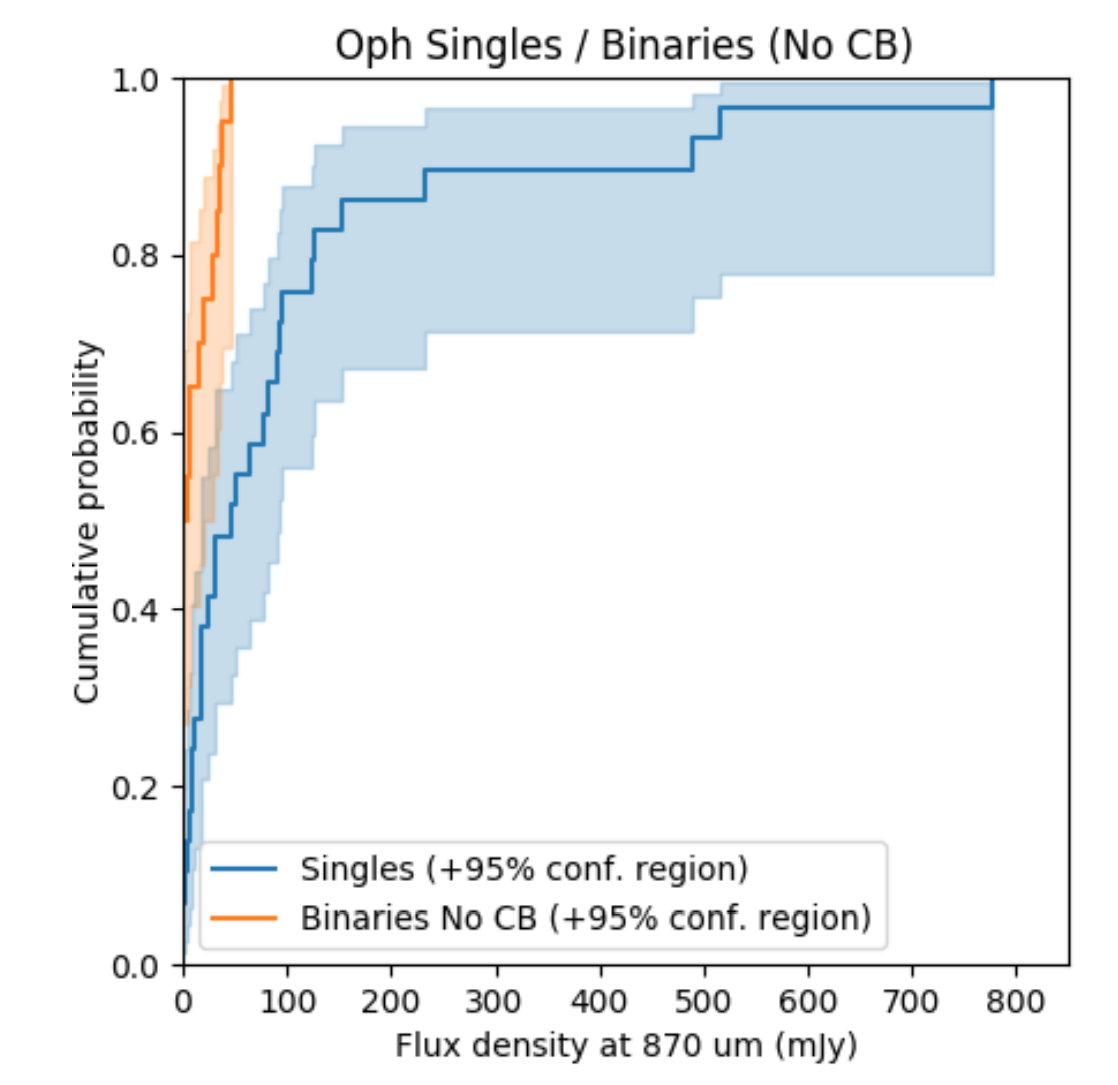
\includegraphics[width=0.33\linewidth]{cox17_rhoOph-singles-bins.png}}%
   \subcaptionbox{CO abundances}{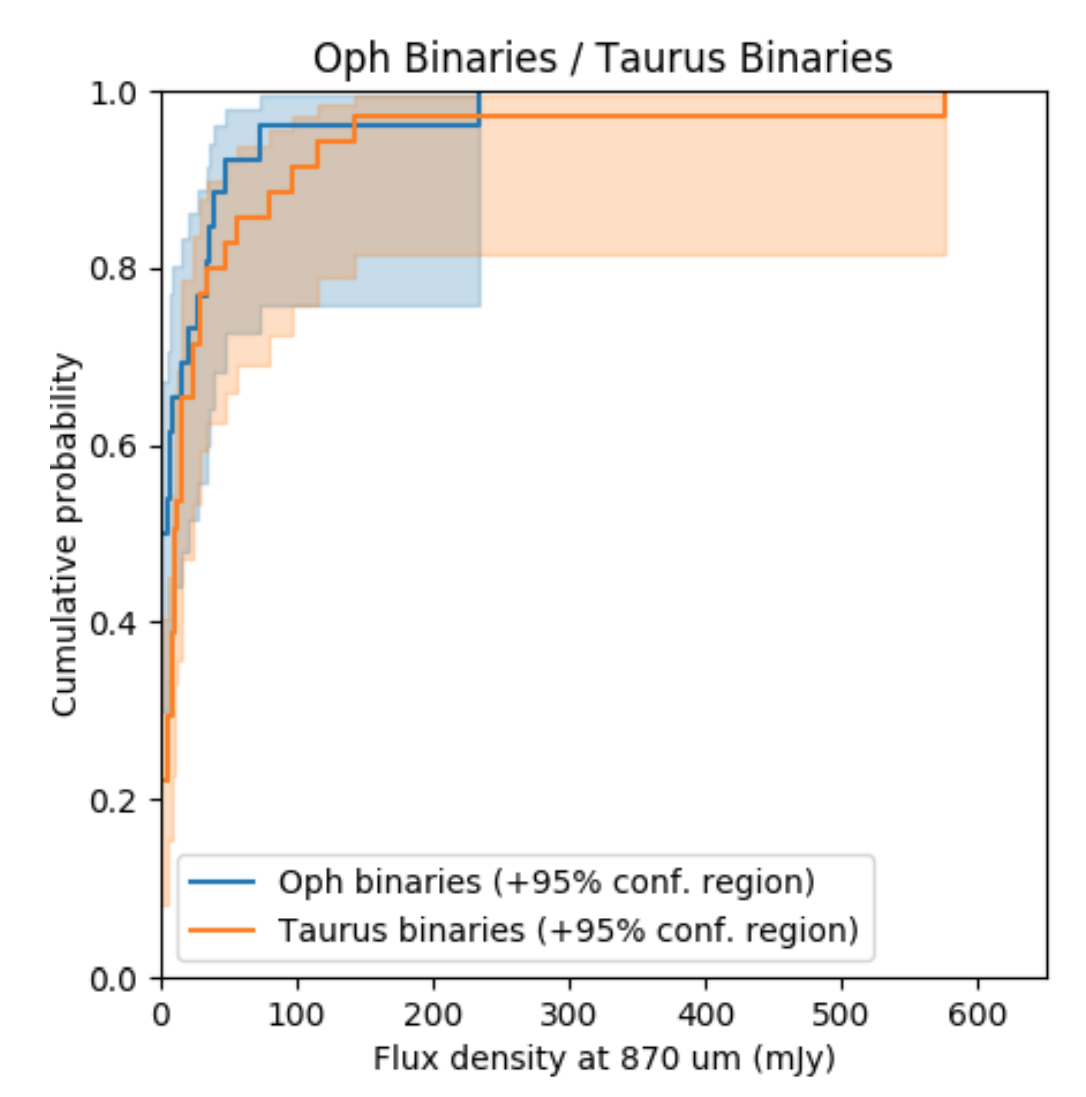
\includegraphics[width=0.33\linewidth]{cox17_taurus-rhhOph-bins.png}}%
   \hspace*{\fill}%
   \caption{\citet{Cox2017} showed that disks in binary systems in $\rho$ Ophiucus have systematically lower fluxes than both isolated disks in the region and disks in binaries in Taurus \citep[from]{Harris2012}.}
   \label{fig:rhoOph_binaries}
 \end{figure}



Comparing the present study's binary pair, however, immediately shows that its disks are neither faint nor small, neither in comparison to the disks in those surveys or to the disks in the survey that it was a part of. However, this is not really out of line from the morphological patterns presented in the surveys above since, at 440 au, the projected separation of these disks is enough to put them beyond the reach of the most significant mass and radius truncations that closer binaries undergo.






\section{Implications}
% - The thing that’s really missing from the discussion is a conversation about what this all means.  *Why* might the similarities/differences between your disk and Sam’s, or your disk and the ones in low-mass SFRs exist?  I think you will be able to write it a lot better once you have expanded your reading beyond just Catherine Walsh’s modeling.  What factors do the modelers predict should affect the chemistry of these disks?  How are these factors related to environment?  To what extent might they be influenced by binarity?  







% REWORK: "Yes, very speculative.  How about mentioning some other possibilities?  For example, if the central stars are different spectral types, that could affect the photochemistry, or different initial disk masses/optical depths could affect how the disks evolve, or planets… try thinking of some more possibilities, and dig into the literature to find some references (they are out there!)"
\citet{Williams2014} posit that wide binaries (systems with separations $\geq$ 300 au), such as this one, do not form in the same initial cloud structures\footnote{Jonathan doesn't actually put any references on this; I have no idea where he got it from. He just puts in references to other papers looking at misaligned binaries}. If this is the case, the notable differences in abundances between disk A and disk B could indicate that the disks in d253-1536 formed separately in clouds with different chemical compositions before joining together later. This is, of course, entirely speculative, but is a possibility.
% REWORK: Re the footnote: "Hm, I’m not sure either, but I would take a look at Robert Harris’s PhD thesis papers on binaries with the SMA as a starting point — check his intro and discussion for relevant references.  Could also check the more recent Akeson/Jensen papers on binaries with ALMA for some relevant intro/discussion material.  Would be good to expand upon this point in the discussion."


















% The End
